\documentclass[letterpaper, 12pt]{article}
\usepackage[margin=1in]{geometry}
\usepackage{graphicx}
\usepackage{listings}
\graphicspath{{images/}{../Template/images/}}
\lstset{language=[Motorola68k]assembler,basicstyle=\ttfamily,frame=single}

\newcommand{\hwnumber}{Lab 1}
\newcommand{\duedate}{September 14th, 2015}

\newcommand{\capper}{\begin{flushright}Aviles, Jean-Ralph \\ EEL3744 \\ Section 1539 \\ \duedate{} \\ \hwnumber{}\end{flushright}}

\begin{document}
\capper{}
\section*{Questions}
\begin{enumerate}
\item What memory location should \textbf{.DSEG} start? Why? \\
\hspace*{8pt} According to the manual, the data segment should start at memory location \textbf{0x2000} because that is the way the architecture was designed.
\item What registers can be used to read from program memory (flash)? \\
\hspace*{8pt} Only the Z register according to the documentation\ldots
\begin{quote}
The Z-register can also be used as an address pointer to read from and/or write
to the flash program memory, signature rows, fuses, and lock bits.
\end{quote}
\item What is the difference between program and data memory? \\
\hspace*{8pt} The biggest difference is how big the pages are; the flash's page size is one word (two bytes) while the data memory's page size is one byte. Also the Z register is used to access Flash memory locations. They also differ in how they are organized and what sections are located within each, a more detailed list is available in the manual. Data memory also affords 1 cycle access times which may be important.
\end{enumerate}
\section*{Problems Encountered}
In writing the assembly code, the most frustrating thing was that the program memory is indexed by word while the reset of the memory map is indexed by byte. This made it extremely difficult to find where I had .ORG'd TABLE1.
\section*{Future Work/Applications}
This gave me a good intro to writing assembly for the Atmel. I have written MIPS and x86 assembly before but its nice that I'm going to have an actual Atmel board to test my assembly instructions on.
\pagebreak[4]
\section*{Pseudocode/Flowcharts}
\subsection*{Part B + C | Debug a Simulated ASM project}
\begin{center}
\begin{lstlisting}
NUL := 0x0
LOWERBOUND := 0x21
UPPERBOUND := 0x40
Table1 := 0x4230
Table2 := 0x2B10
SRC := Address(Table1) - 1
DEST := Address(Table2)
DO
	SRC = SRC + 1
	IF DATA(SRC) <= LOWERBOUND OR DATA(SRC) > UPPERBOUND
	THEN
		DATA(DEST) = DATA(SRC)
		DEST = DEST + 1
	ENDIF
ENDDO
WHILE DATA(SRC) IS NOT NUL
\end{lstlisting}
\end{center}
\section*{Programs}
\subsection*{Part B and C -- Code}
\lstinputlisting{code/Lab1_b_ja.asm}
\section*{Appendix}
\subsection*{Part A - Screenshot}
\begin{center}
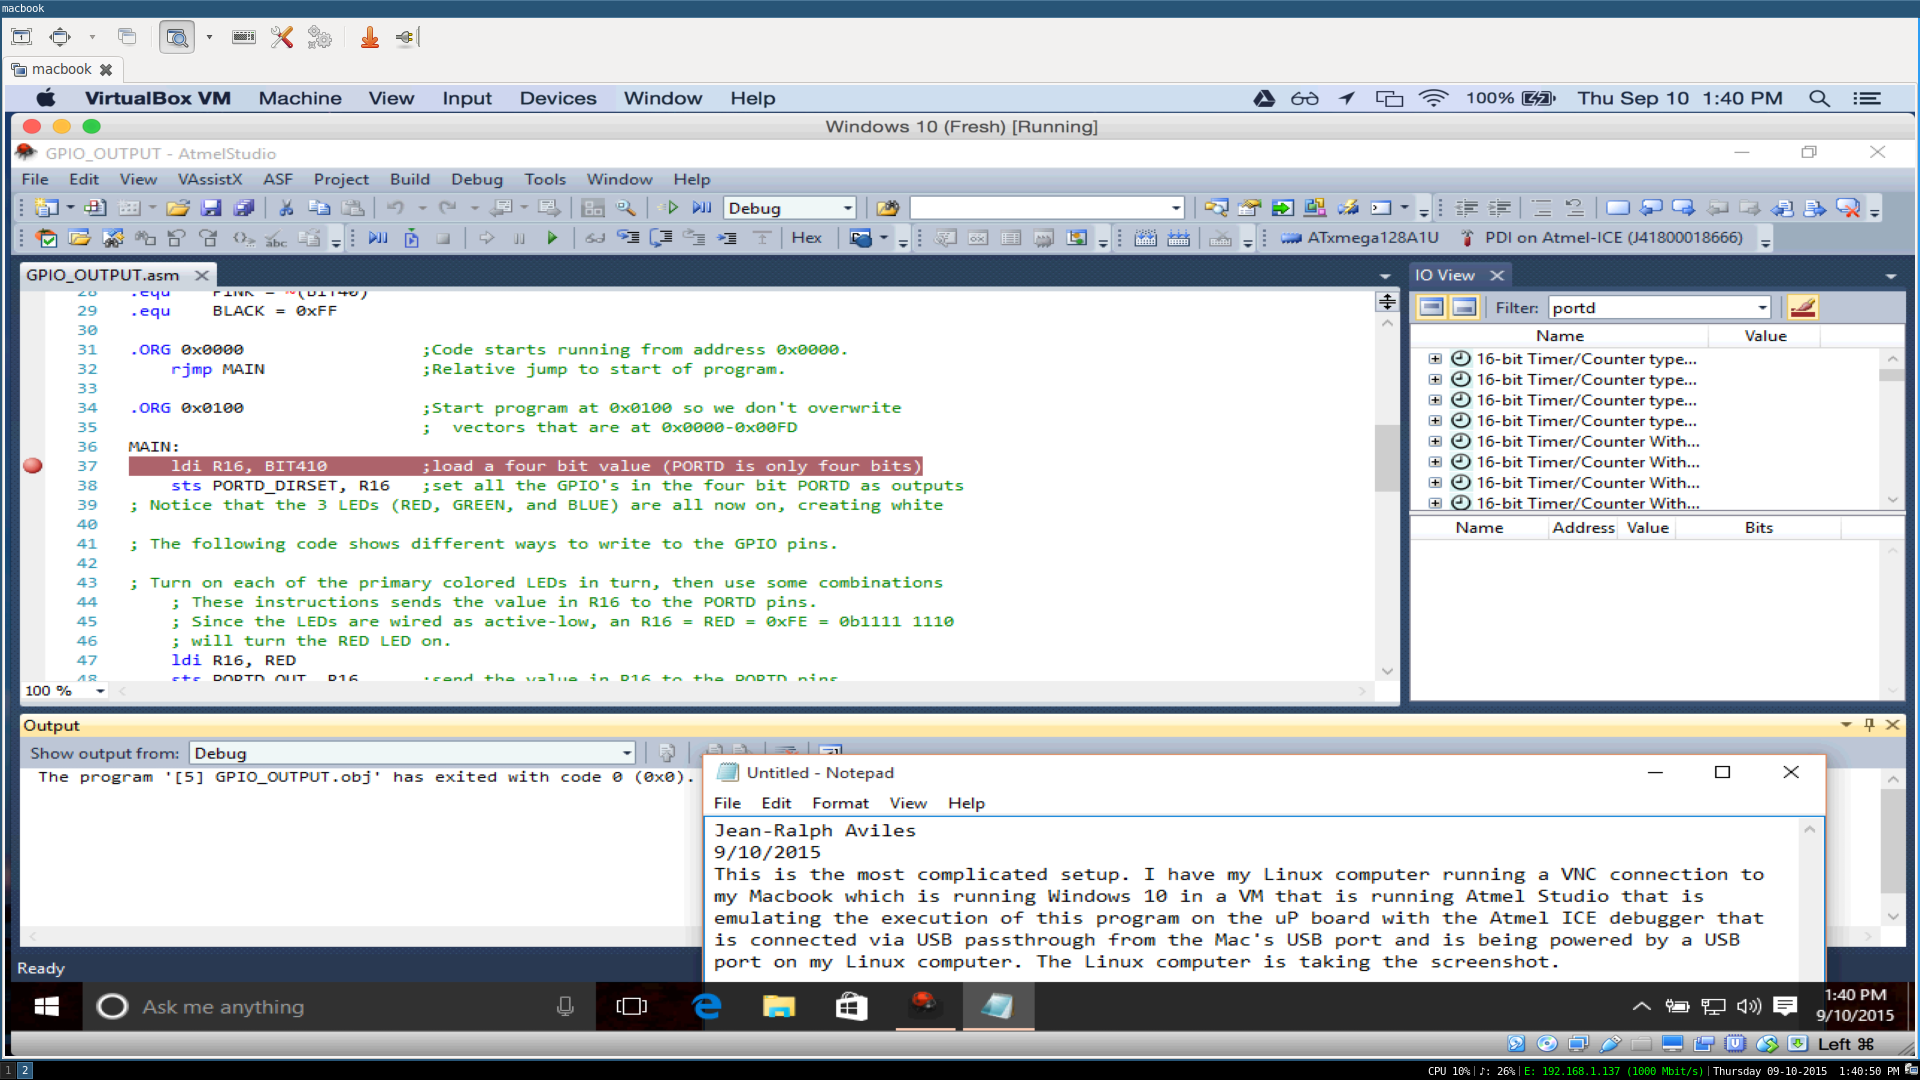
\includegraphics[width=1.0\textwidth,keepaspectratio=true]{emulation}
\end{center}
\subsection*{Part B - Screenshot}
\begin{center}
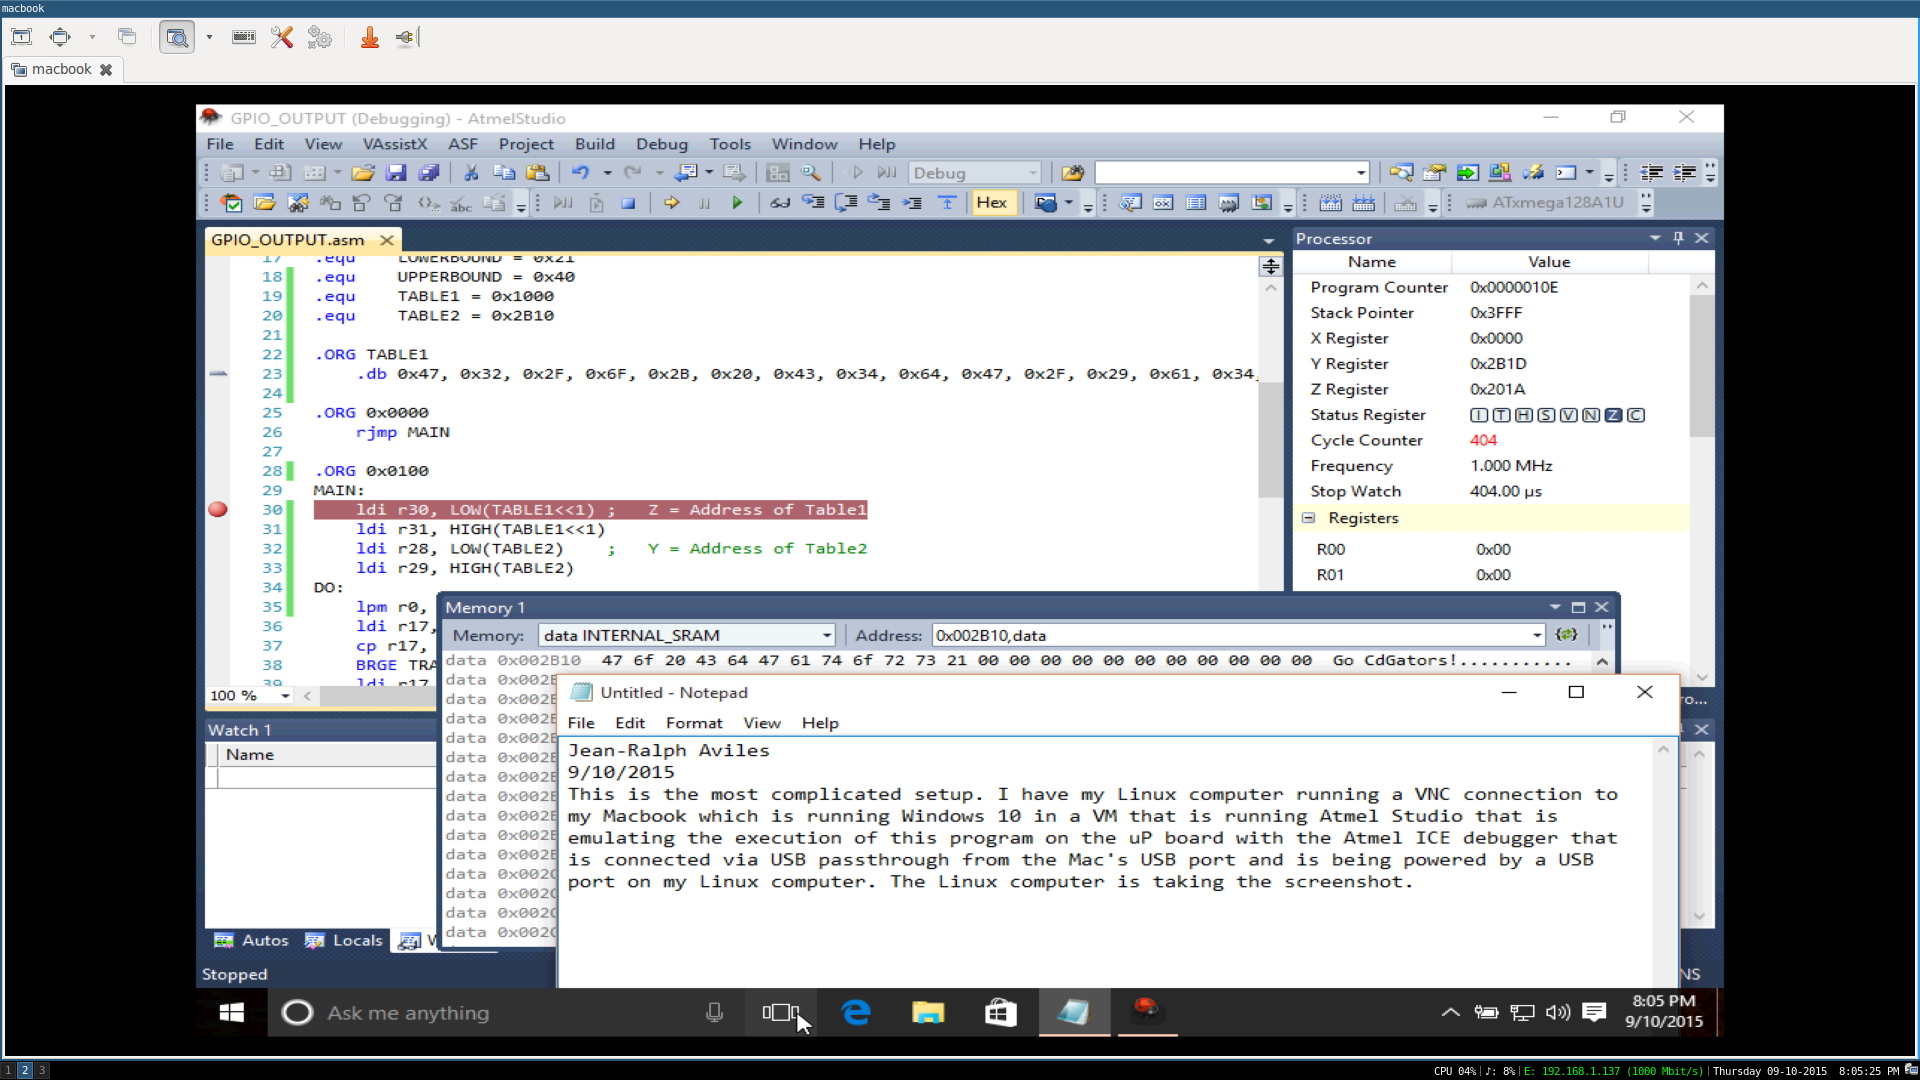
\includegraphics[width=1.0\textwidth,keepaspectratio=true]{debug_simulated}
\end{center}
\subsection*{Part C - Screenshot}
\begin{center}
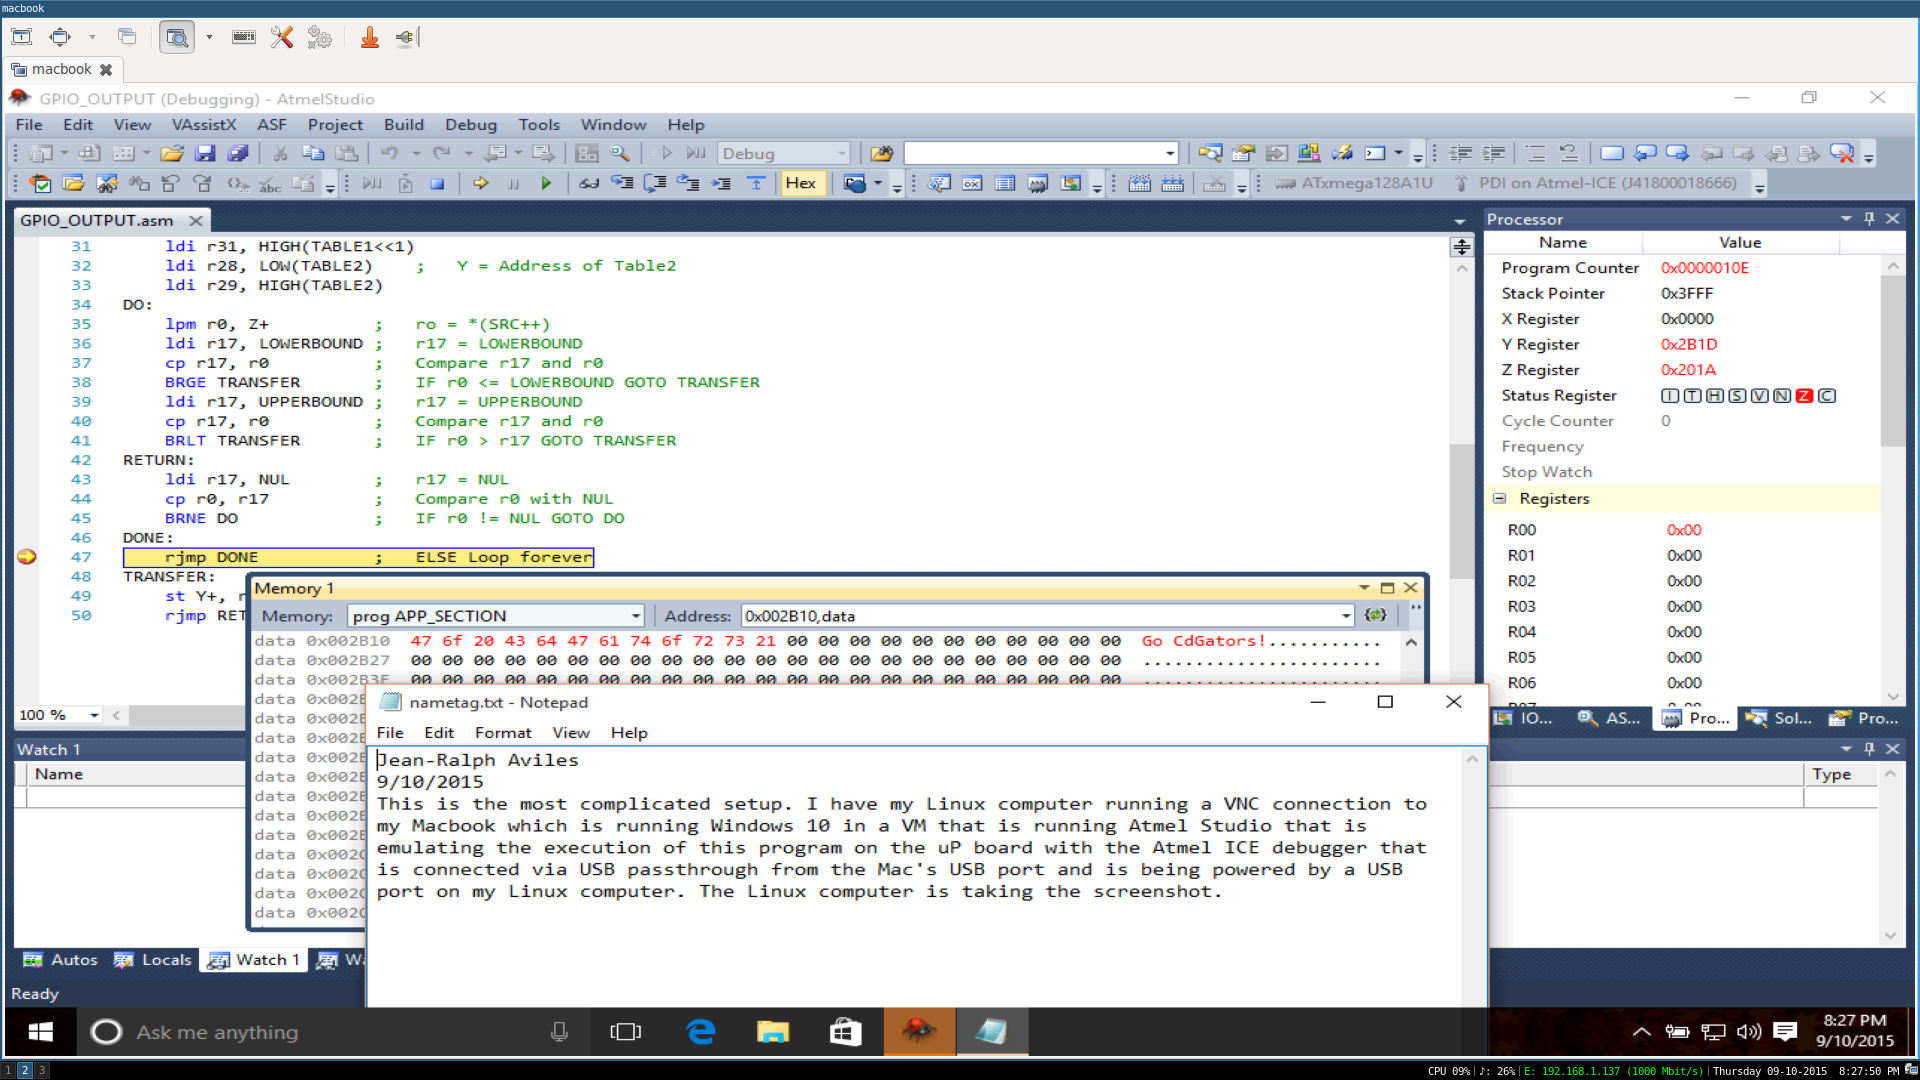
\includegraphics[width=1.0\textwidth,keepaspectratio=true]{debug_emulated}
\end{center}
\end{document}
